\documentclass[oneside,14pt]{extarticle}
\usepackage{cmap}
\usepackage[utf8]{inputenc}
\usepackage{longtable}
\usepackage[english,ukrainian]{babel}
\usepackage{graphicx}
\usepackage{geometry}
\usepackage{listings}
\usepackage{float}
\usepackage{amsmath}
\usepackage{subfig}
\usepackage{tempora}
\renewcommand{\arraystretch}{1.5}
\usepackage{titlesec}
\titleformat{\section}
{\centering\Large\bfseries}{\thesection}{1em}{} % Centered, large, bold font
\geometry{
	a4paper,
	left=20mm,
	right=20mm,
	top=15mm,
	bottom=15mm,
}
\lstset{
	language=c,
	tabsize=4,
	keepspaces,
	showstringspaces=false,
	frame=single,
	breaklines,
	language=C,
}
\graphicspath{ {./pictures} }
\setlength{\parindent}{4em}

\newcommand\subject{Якість програмного забезпечення та тестування}
\newcommand\lecturer{доцент кафедри ПЗ\\Фоменко А.В.}
\newcommand\teacher{асистент кафедри ПЗ\\Джумеля Е.А.}
\newcommand\mygroup{ПЗ-42}
\newcommand\lab{8}
\newcommand\theme{Модульне тестування}
\newcommand\purpose{Закріпити теоретичні знання шляхом написання модульних
	тестів}

\begin{document}
\begin{normalsize}
	\begin{titlepage}
		\thispagestyle{empty}
		\begin{center}
			\textbf{МІНІСТЕРСТВО ОСВІТИ І НАУКИ УКРАЇНИ\\
				НАЦІОНАЛЬНИЙ УНІВЕРСИТЕТ "ЛЬВІВСЬКА ПОЛІТЕХНІКА"}
		\end{center}
		\begin{flushright}
			\textbf{ІКНІ}\\
			Кафедра \textbf{ПЗ}
		\end{flushright}
		\vspace{80pt}
		\begin{center}
			\textbf{ЗВІТ}\\
			\vspace{10pt}
			до лабораторної роботи № \lab\\
			\textbf{на тему}: <<\textit{\theme}>>\\
			\textbf{з дисципліни}: <<\subject>>
		\end{center}
		\vspace{80pt}
		\begin{flushright}
			
			\textbf{Лектор}:\\
			\lecturer\\
			\vspace{28pt}
			\textbf{Виконали}:\\
			
			студенти групи \mygroup\\
			Коваленко Д.М.\\
			Снісар В.І.\\
			Баран В.Б.\\
			\vspace{28pt}
			\textbf{Прийняла}:\\
			
			\teacher\\
			
			\vspace{28pt}
			«\rule{1cm}{0.15mm}» \rule{1.5cm}{0.15mm} 2024 р.\\
			$\sum$ = \rule{1cm}{0.15mm}……………\\
			
		\end{flushright}
		\vspace{\fill}
		\begin{center}
			\textbf{Львів – 2024}
		\end{center}
	\end{titlepage}
		
	\begin{description}
		\item[Тема.] \theme.
		\item[Мета.] \purpose.
	\end{description}

    \section*{Лабораторне завдання}
    \begin{enumerate}
    	\item Відкрити приклад з тестами, ознайомитись з ними, виконати з використанням XUnit.
    	\item Створити новий проект модульних тестів у Visual Studio 2008 (використовуючи XUnit або Microsoft unit testing framework)
    	.
    	\item Написати 10 модульних тестів для одного з власних класів.
    	Написати 10 модульних тестів для одного з власних класів.
    \end{enumerate}
	\section*{Хід роботи}
	\subsection*{Код тестів}
	\begin{lstlisting}
#[cfg(test)]
mod tests {
	use super::*;
	
	#[test]
	fn initializes_empty_diagram_correctly() {
		let diagram = Diagram::new();
		assert!(diagram.is_empty());
	}
	
	#[test]
	fn adds_actor_to_diagram() {
		let mut diagram = Diagram::new();
		diagram.add_actor("User");
		assert_eq!(diagram.actors.len(), 1);
	}
	
	#[test]
	fn creates_association_between_actors() {
		let mut diagram = Diagram::new();
		diagram.add_actor("User");
		diagram.add_actor("Admin");
		let result = diagram.add_association("User", "Admin");
		assert!(result.is_ok());
	}
	
	#[test]
	fn handles_duplicate_actor_names() {
		let mut diagram = Diagram::new();
		diagram.add_actor("User");
		let result = diagram.add_actor("User");
		assert!(result.is_err());
	}
	
	#[test]
	fn validates_use_case_title_not_empty() {
		let use_case = UseCase::new("");
		assert!(use_case.is_invalid());
	}
	
	#[test]
	fn checks_inclusion_relationship_exists() {
		let mut diagram = Diagram::new();
		let use_case1 = diagram.add_use_case("Login");
		let use_case2 = diagram.add_use_case("Authenticate");
		let result = diagram.add_inclusion(use_case1, use_case2);
		assert!(result.is_some());
	}
	
	#[test]
	fn verifies_class_diagram_inheritance() {
		let mut class_diagram = ClassDiagram::new();
		class_diagram.add_class("Parent");
		let result = class_diagram.add_inheritance("Child", "Parent");
		assert!(result.is_some());
	}
	
	#[test]
	fn prevents_circular_inheritance() {
		let mut class_diagram = ClassDiagram::new();
		class_diagram.add_class("A");
		class_diagram.add_class("B");
		class_diagram.add_inheritance("A", "B");
		let result = class_diagram.add_inheritance("B", "A");
		assert!(result.is_err());
	}
	
	#[test]
	fn checks_diagram_export_format() {
		let diagram = Diagram::new();
		let export = diagram.export();
		assert!(export.contains("json"));
	}
	
	#[test]
	fn verifies_sequence_diagram_message_order() {
		let mut sequence = SequenceDiagram::new();
		sequence.add_message("User", "LoginService", "Authenticate");
		sequence.add_message("LoginService", "User", "Success");
		let is_ordered = sequence.check_order();
		assert!(is_ordered);
	}
}
	\end{lstlisting}
	
	\begin{figure}[H]
		\centering
		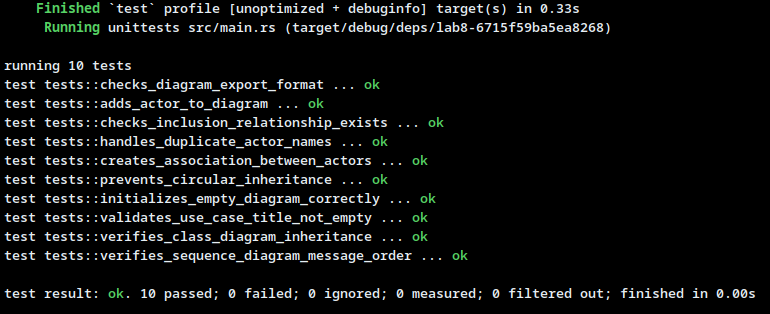
\includegraphics[width=\columnwidth]{1}
		\caption{Результат тестування}
	\end{figure}
	
	\section*{Висновки}
	Під час виконання лабораторної роботи розроблено 10 тестів для модуля проектування, які перевіряють основні функції: ініціалізацію діаграм, додавання акторів, створення зв'язків, обробку дубльованих імен та перевірку назв. Тести також охоплюють спадкування у класах, формат експорту та порядок повідомлень у діаграмах послідовностей, що забезпечує стабільність модуля.
	    
\end{normalsize}
\end{document}
